% \documentclass[aspectratio=169]{beamer} % includes \pause in render
\documentclass[aspectratio=169, handout]{beamer} % do not include \pause in render

\usetheme[neutralbackground]{uniamntf}

\title[Computer aided calculations]{\vspace{-2em}Computer aided Analytical Calculations for Physical Many-Body Problems}
\subtitle{ - Project Work Presentation - }

\author{Jonas Kell}
\institute[TP III]{Chair for theoretical Physics III}

\date[01.05.2024]{$15^{\text{th}}$ of Mai 2024}

\acknowledgement{
    Jonas Kell\\
    Augsburg University\\
    jonas.kell@student.uni-augsburg.de\\
    www.uni-augsburg.de
}

\newcommand{\blankfootnote}[1]{%
\let\thefootnote\relax\footnotetext{#1}%
}
\newcommand{\tab}{%
\,\,\,\,
}

% bibtex/biber
\usepackage[backend=biber, style=phys, biblabel=brackets]{biblatex} % citations with "modern" backend and an physics-accepted citation style
\addbibresource{literature.bib}

\newenvironment{wideitemize}{\itemize\addtolength{\itemsep}{0.3em}}{\enditemize}

%! notes control

%\setbeameroption{hide notes} % Only slides
%\setbeameroption{show only notes} % Only notes
\setbeameroption{show notes on second screen=right} % Both, use for pympress mode

% presentation tool https://github.com/Cimbali/pympress
% run: pympress project-work-presentation.pdf 

%! notes control

\begin{document}
    \begin{frame}[t,plain] 
        \maketitle
    \end{frame}

    \note[enumerate]{
        \item Welcome
        \item Presentation of "Project Work" (Projektarbeit)
        \item Runs parallel to the "Practical Training" (Fachpraktikum)
        \item Presentation in this Group-Slot
    }

    \begin{frame}
        \frametitle{Outline}
        \tableofcontents[pausesections] % pause toc before each section
        % \tableofcontents % all toc at once

        % toc notes do need to live inside the frame, to appear on all animated slides
        \note[item] {
            Introduction of theme worked on in Project-Work, Practical Training and Master Thesis
            \begin{itemize}
                \item The mathematical Problem of Many-Body Physics
                \item The computational/notational problem of "doing maths easily"
            \end{itemize}
        }
        \note[item] {
            What was there to make it easier (Off the shelf solutions)
        }
        \note[item] {
            What I did:
            \begin{itemize}
                \item Math Manipulator
                \item Tricks to use to improve your Python
                \item Latex for presentations
            \end{itemize}
        }
        \note[item] {
            Gist: after I (somewhat of a computer scientist by trade) learned the process of being a theoretical physicist, I want to bring back some tools/workflows to maybe improve someones life here at TP III  
        }
    \end{frame}


    When performing time-evolution with a perturbative approach, one ought to watch out for resonances.
In the case of degenerate energy solutions, so-called \emph{secular terms} \cite{secularTermsPerturbation} might be introduced, if non-degenerate perturbation theory is used to find the solution to a degenerate problem. 
Often inaccuracies manifest as linear terms in a function where only oscillating terms would be expected.
The linear term constantly grows over time, guaranteeing the approximation is only valid for short times and then diverges further and further from the exact solution.

For the examined Hamiltonian the first occurrence of such terms can be spotted in the second order cumulant expansion of the Hamiltonian.
\autoref{eq:time-ordered-integral-part1} and \autoref{eq:time-ordered-integral-part2} specifically list extra solutions for the cases where the two energies are the same.
This resonance causes a linear term to appear in the expansion, while all other pre-factors so far were complex exponentials -- meaning they are oscillating.

The idea to combat this is to replace the perturbative parameters that were calculated analytically with variational parameters instead.
This has the motive to generate a physically motivated structure, but the fine details of the parameter weights are adjusted by optimization.
E.g. for the \emph{neural-network quantum state} \cite{neuralNetworkQuantumStates} approach, a neural network structure is used to represent a wave-function.
Reason for this being the hope that the exponentially complicated wave-function can be expressed as a \glqq higher truth\grqq{} only requiring few parameters to describe a seemingly complicated wave-function.
While it would be basically impossible to always find the few-parameter-solution, \emph{approximating} it close enough with optimization akin to machine-learning should be a suitable replacement.

The following section aims to achieve better approximations than the ones found by cumulant expansion by letting the parameters be optimized during the step to reflect the situation more closely.
    As stated in \fullref{sec:theory}, some of the analytical calculations involving ladder-operators have been performed with the tool \emph{Math-Manipulator} \cite{selfMathManipulator}.
This tool was purpose-built to play with operators, that obey specific commutation-relations, in a way which lies in between writing on paper and using a \emph{computer algebra system}.
Originally this started as a passion-project with the purpose of gaining knowledge about \emph{lexing}, \emph{parsing} and the handling of \emph{operator trees} to gain deeper experience with the working of compilers \cite{compilersDragonBook}.
After adding a \LaTeX-renderer and full browser support to minimize the friction of adopting such a new tool into established workflows, it became clear that it could be useful to perform some of the necessary analytical calculations.
Having encountered many exercise-problems with the main focus on ladder-operator commutation-relations over the course of the master curriculum, oftentimes the tediousness of such calculations started to obscure the real lessons of the exercises.
The project tries to establish itself as a low-friction option that fits into manual \glqq on-paper\grqq{} workflows and is yet powerful, extensible and provides reproducible calculations.

Some sections in the practical training report \filepath{\cite{selfDocument}}{/practical-training-latex} are dedicated to outlining the implementation, giving a basic overview of the theoretical backbone and redirecting to further resources.
\filepath{\cite{selfDocument}}{/project-work-presentation} is discussing advantages and disadvantages of classical \glqq on-paper\grqq{} calculation vs. fully strict computer algebra systems.
As both of these reports devote their focus to painting a more detailed picture, there will be no in-depth presentation of the side-project to this thesis here.
In the case of further interest, it is best to follow the linked resources.

As a summarizing statement to gauge the necessity and usefulness of this detour, only the next paragraph should be sufficient.

While there already exist better tools for similar use-cases, the introduction of this new one does not aim to replace, imitate or upstage any of them.
The focus of Math-Manipulator is to position itself as a playground to experiment with the behavior of non-commutative operators and related mathematical objects, while reducing the expense on repetitive manual calculations and providing results that are easier to reproduce.
During the development process and the first-hand usage on an actual scientific problem, it helped making the operator behavior tangible.
Even though the time spent on developing the tool might outweigh the time that would have been necessary for writing down the final version of the calculations, during re-calculations and iterations it already could save many hours.
Furthermore, only having such a consistent iteration cycle made it possible to arrive at the cleanliness of the final presented calculations.
And finally, the stored save-files of the calculations make it possible to share the equations that are not put into the final thesis in a standardized way - without resorting to inclusion of large and complex parts in the appendix and supplementary material.

    \section{Custom Python Scripts (SymPy)}
    \begin{frame}
        \frametitle{Optimization: Difference of V(t) for Hopping}

        \begin{columns}
            \column{0.4\textwidth}
                \begin{itemize}
                    \onslide
                    \item Monte-Carlo sampling requires transition probabilities between "adjacent" states
                    \pause
                    \item These require differences of $\hat{V}^\mathrm{I}(t)$ and $E_0$
                    \pause
                    \item Too many terms for simple evaluation by hand
                    \item Intelligent pre-computation required to speed up processing
                \end{itemize}
            \column{0.4\textwidth}
                \onslide
                \makebox[\textwidth][c]{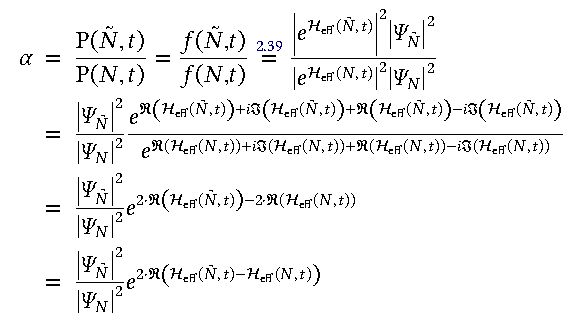
\includegraphics[width=1.3\textwidth]{main-content/python/sampling-probability.pdf}}
                
        \end{columns}

        % notes 
        \onslide % on all slides of frame
        \note[item] {
            "Adjacent" states because from one Monte-Carlo step to the next we require a small change of one or two particle-sites. Could come from hopping or flipping.
        }
        \note[item] {
            The $E_0$ differences are quickly calculated by hand in the report
        }
    \end{frame}

    \begin{frame}
        \frametitle{The process: Difference of V(t) for Hopping}
        
        \hspace{-1cm}
        \makebox[\textwidth][c]{
            \onslide<1->
            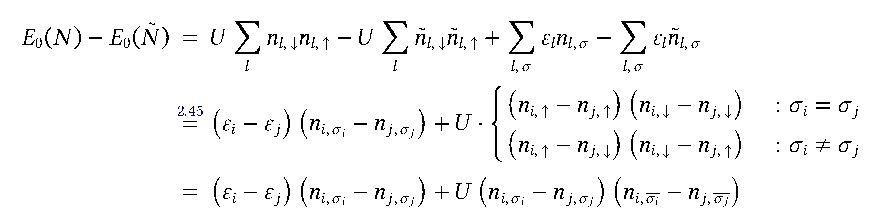
\includegraphics[width=0.7\textwidth]{main-content/python/hopping-e0-example.pdf}
            \onslide<2->
            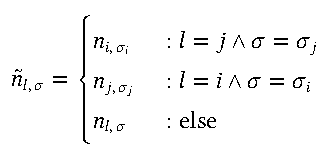
\includegraphics[width=0.28\textwidth]{main-content/python/n-redefinition.pdf}
        }

        \vspace{0.3cm}

        \begin{itemize}
            \onslide<1->
            \item Setup difference
            \onslide<2->
            \item Replace one by appropriate new occupation
            \onslide<3->
            \item Simplify as much as possible
            \item Sum over all possible neighbor combinations
        \end{itemize}

        \vspace{0.1cm}
        
        \onslide<4->
        \textbf{Problem:} number of terms/combinations: $3 \cdot 8 \cdot 4 \cdot 2 = 192$

        % notes 
        \onslide % on all slides of frame
        \note[item] {
            The $V$ differences are $3 \cdot 8 \cdot = 32 \cdot 4 = 96 \cdot 2 = 192$ terms
        }
        \note[item] {
            The process is relatively straight forward:
            \begin{itemize}
                \item write down the terms
                \item replace
                \item simplify difference
            \end{itemize}
        }
        \note[item] {
            Still quite complicated and a lot of work, but: 
            \begin{itemize}
                \item way faster to write bacuse non-repetetive logic
                \item verifiably correct calculations
                \item multiple times re-done on changes to underlying code, each time only took seconds
                \item sometimes brute-force NEEDS to work, before optimization can be found
            \end{itemize}
        }
    \end{frame}

    \begin{frame}
        \frametitle{Script-Generation: Difference of V(t) for Hopping}
        
        \begin{block}{Generating Script}
            \href{https://github.com/jonas-kell/master-thesis-code/blob/master/calculation-helpers/simplificationtermhelper.py}{simplificationtermhelper.py}
        \end{block}

        \vspace{1cm}

        \begin{block}{Generated Script}
            \href{https://github.com/jonas-kell/master-thesis-code/blob/master/computation-scripts/analyticalcalcfunctions.py}{analyticalcalcfunctions.py}
        \end{block}

        % notes 
        \onslide % on all slides of frame
        \note[item] {
            \texttt{simplificationtermhelper.py} script to generate the script
        }
        \note[item] {
            \texttt{analyticalcalcfunctions.py} script is generated and used in the code
        }
        \note[item] {
            Generated file: 1556 lines, script that generates: 534 lines
        }
        \note[item] {
            Show the script that generates/is generated $\rightarrow$ simplification with Sympy \item Parallel to computer-science practice "Vendored" code
        }
    \end{frame}
    \section{Presentations? - Custom Beamer Template}
    \begin{frame}{Beamer: LaTeX way of writing Presentations}
        \begin{itemize}
            \item Write presentations like your papers/thesis in \LaTeX \pause
            \item Reuse formulas/images/code/sources \pause
            \item Consistent style \& references    \pause
            \item Version control    \pause
            \item Easier collaboration
        \end{itemize}

        \blankfootnote{Beamer \cite{beamerPackageCtan} \tab{} Template \cite{selfBeamerTemplateMNTF}}
    \end{frame}

    \note[enumerate]{
        \item Re-use tooling, editor, setup (even this on overleaf alone much better that shared powerpoint presentation)
        \item This presentation, report and thesis all live in one git-repository and share resources
        \item Everything I ever work on is hosted in Git.
        \begin{itemize}
            \item Without Version Control it is no longer possible for me to work effectively
            \item Every workflow is massively ensured by it
            \item Also for single-person work, but built in collaboration, synchronization and backup
        \end{itemize}
    }

    \begin{frame}{Minimal example for beamer presentation}
        \begin{columns}
            \column{0.4\textwidth}
                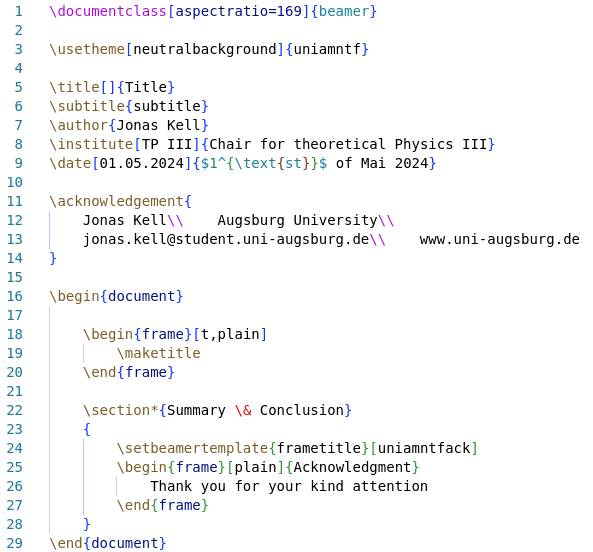
\includegraphics[width=1.1\textwidth]{./beamer-minimal-example/code.png}
            \column{0.4\textwidth}
                
\includegraphics[width=0.9\textwidth]{./beamer-minimal-example/result.png}
        \end{columns}
    \end{frame}

    \note[enumerate]{
        \item 29 lines gets you a basic presentation
        \item First time very much slower as putting together by hand in PowerPoint
        \item If you want to do crazy stuff, possible but really hard
        \item Actually quite a timesaver when you have an example/template to work of and do not require crazy levels of features
        \item When it works, perfectly portable (just a pdf), high performant and versatile (output rendering of presentation, notes, animations from one source)
    }


    \section*{Summary \& Conclusion}
    {
        \setbeamertemplate{frametitle}[uniamntfack] % use the acknowledgment-style for this slide
        \begin{frame}[plain]{Acknowledgment}
            \vspace{1cm}

            Thank you for your kind attention\\

            \vspace{1cm}
            \makebox[0.4\textwidth][c]{
                
\includegraphics[width=0.3\textwidth]{extra-slides/qr-github.png}
            }
        \end{frame}
    }

    \note[enumerate]{
        \item Thank you for your kind attention
        \item All tools and other resources are referenced in the presentation
        \item You can also find everything on my Github
    }

    \begingroup % group to not count pages from here
        \begin{frame}[allowframebreaks,noframenumbering]
            \frametitle{References}
            \nocite{*}
            \printbibliography[title={Bibliography}]
        \end{frame}
        
        \section*{Extra slides}
            
\begin{frame}[noframenumbering]{Extra Plots: Overview}
    \begin{itemize}
        \item \hyperlink{plot:exact-comparison}{Exact comparison density matrix}
        \item \hyperlink{plot:energy-variance}{First orders: energy and variance comparison}
        \item \hyperlink{plot:j-sweep}{J parameter sweep}
        \item \hyperlink{plot:mc-convergence}{Monte Carlo sampling convergence}
        \item \hyperlink{plot:runtime-comparison}{Runtime validation}
    \end{itemize}
\end{frame}

\begin{frame}[noframenumbering]{Exact Comparison: Concurrence}
    \label{plot:exact-comparison}
    \vspace{-0.4cm}
    \makebox[\textwidth][c]{\includegraphics[height=.8\paperheight]{./../thesis-latex/plotgeneration/concurrence-from-spin/concurrence-comparison.pdf}}
    \note[item]{
        Concurrence comparison of small system with exact calculations and comparison thereof
    }
    \note[item]{
        See extreme boost of second order 
    }
\end{frame}
\begin{frame}[noframenumbering]{Exact Comparison: Purity}
    \vspace{-0.4cm}
    \makebox[\textwidth][c]{\includegraphics[height=.8\paperheight]{./../thesis-latex/plotgeneration/concurrence-from-spin/purity-comparison.pdf}}
    \note[item]{
        Purity measurements for the graph of the measurement from one page before
    }
\end{frame}
\begin{frame}[noframenumbering]{Exact Comparison: Pauli Measurements}
    \vspace{-0.6cm}
    \makebox[\textwidth][c]{\includegraphics[height=.83\paperheight]{./../thesis-latex/plotgeneration/concurrence-from-spin/pauli-measurements.pdf}}
    \note[item]{
        Portrait mode format, because extracted from the thesis. 
    }
    \note[item]{
        You can see what a problem the z-contributions are
    }
\end{frame}

\begin{frame}[noframenumbering]{First Orders: Energy Comparison}
    \label{plot:energy-variance}
    \vspace{-0.4cm}
    \makebox[\textwidth][c]{\includegraphics[height=.8\paperheight]{./../thesis-latex/plotgeneration/energy-variance/energy.pdf}}
    \note[item]{
        Second picture zoomed in
    }
\end{frame}
\begin{frame}[noframenumbering]{First Orders: Variance Comparison}
    \vspace{-0.4cm}
    \makebox[\textwidth][c]{\includegraphics[height=.8\paperheight]{./../thesis-latex/plotgeneration/energy-variance/variance.pdf}}
    \note[item]{
        Second picture zoomed in
    }
\end{frame}

\begin{frame}[noframenumbering]{J-Sweep: Current Border}
    \label{plot:j-sweep}
    \vspace{-0.4cm}
    \makebox[\textwidth][c]{\includegraphics[height=.8\paperheight]{./../thesis-latex/plotgeneration/j-sweep/current-border.pdf}}
    \note[item]{
        Logarithmic plot
    }
    \note[item]{
        Measurements show the trend of the convergence of the relative error for small perturbations
    }
    \note[item]{
        Depends on the observable though, still
    }
\end{frame}
\begin{frame}[noframenumbering]{J-Sweep: Current Center}
    \vspace{-0.4cm}
    \makebox[\textwidth][c]{\includegraphics[height=.8\paperheight]{./../thesis-latex/plotgeneration/j-sweep/current-center.pdf}}
\end{frame}
\begin{frame}[noframenumbering]{J-Sweep: Single Occupation Center}
    \vspace{-0.4cm}
    \makebox[\textwidth][c]{\includegraphics[height=.8\paperheight]{./../thesis-latex/plotgeneration/j-sweep/single-occ-center.pdf}}
\end{frame}
\begin{frame}[noframenumbering]{J-Sweep: Double Occupation Border}
    \vspace{-0.4cm}
    \makebox[\textwidth][c]{\includegraphics[height=.8\paperheight]{./../thesis-latex/plotgeneration/j-sweep/double-occ-border.pdf}}
\end{frame}

\begin{frame}[noframenumbering]{Monte Carlo Convergence: Occupation}
    \label{plot:mc-convergence}
    \vspace{-0.4cm}
    \makebox[\textwidth][c]{\includegraphics[height=.8\paperheight]{./../thesis-latex/plotgeneration/monte-carlo-variance-test/occupation.pdf}}
    \note[item]{
        Well as we can see, the appriximation converges as the variance gos to zero
    }
\end{frame}
\begin{frame}[noframenumbering]{Monte Carlo Convergence: Occupation}
    \vspace{-0.4cm}
    \makebox[\textwidth][c]{\includegraphics[height=.8\paperheight]{./../thesis-latex/plotgeneration/monte-carlo-variance-test/spin-current.pdf}}
\end{frame}

\begin{frame}[noframenumbering]{Runtime Validation}
    \label{plot:runtime-comparison}
    \vspace{-0.4cm}
    \makebox[\textwidth][c]{\includegraphics[height=.8\paperheight]{./../thesis-latex/plotgeneration/runtime-complexity/runtime.pdf}}
\end{frame}

% \makebox[\textwidth][c]{\includegraphics[height=.8\paperheight]{./../thesis-latex/plotgeneration/vcn-eff-stepsize/}}
% \makebox[\textwidth][c]{\includegraphics[height=.8\paperheight]{./../thesis-latex/plotgeneration/vcn-energy-conservation/}}
% \makebox[\textwidth][c]{\includegraphics[height=.8\paperheight]{./../thesis-latex/plotgeneration/vcn-square-comparison/}}
% \makebox[\textwidth][c]{\includegraphics[height=.8\paperheight]{./../thesis-latex/plotgeneration/vcn-square-small/}}
% \makebox[\textwidth][c]{\includegraphics[height=.8\paperheight]{./../thesis-latex/plotgeneration/system-size-dependency/}}

% \begin{frame}[noframenumbering]{}
%     \label{plot:exact-comparison}
%     \vspace{-0.4cm}
%     \note[item]{
%     }
% \end{frame}
    \endgroup

\end{document}
